% ####################################################################
% Basic configuration of Beamera class and Jagiellonian theme
% ####################################################################
\RequirePackage[l2tabu, orthodox]{nag}



\ifx\PresentationStyle\notset
  \def\PresentationStyle{dark}
\fi



% Options: t - align frame text to the top.
\documentclass[10pt,t]{beamer}
\mode<presentation>
\usetheme[style=\PresentationStyle]{jagiellonian}




% ######################################
% Procesing configuration files of Jagiellonian theme located
% in the directory "preambule"
% ######################################
% Configuration for polish language
% Need description
\usepackage[polish]{babel}
% Need description
\usepackage[MeX]{polski}



% ------------------------------
% Better support of polish chars in technical parts of PDF
% ------------------------------
\hypersetup{pdfencoding=auto,psdextra}

% Package "textpos" give as enviroment "textblock" which is very usefull in
% arranging text on slides.

% This is standard configuration of "textpos"
\usepackage[overlay,absolute]{textpos}

% If you need to see bounds of "textblock's" comment line above and uncomment
% one below.

% Caution! When showboxes option is on significant ammunt of space is add
% to the top of textblock and as such, everyting put in them gone down.
% We need to check how to remove this bug.

% \usepackage[showboxes,overlay,absolute]{textpos}



% Setting scale length for package "textpos"
\setlength{\TPHorizModule}{10mm}
\setlength{\TPVertModule}{\TPHorizModule}


% ---------------------------------------
% Packages written for lectures "Geometria 3D dla twórców gier wideo"
% ---------------------------------------
% \usepackage{./Geometry3DPackages/Geometry3D}
% \usepackage{./Geometry3DPackages/Geometry3DIndices}
% \usepackage{./Geometry3DPackages/Geometry3DTikZStyle}
% \usepackage{./ProgramowanieSymulacjiFizykiPaczki/ProgramowanieSymulacjiFizykiTikZStyle}
% \usepackage{./Geometry3DPackages/mathcommands}


% ---------------------------------------
% Importing TikZ's libraries
% ---------------------------------------
\usetikzlibrary{arrows.meta}
\usetikzlibrary{positioning}





% % Configuration package "bm" that need for making bold symbols
\newcommand{\bmmax}{0}
\newcommand{\hmmax}{0}
\usepackage{bm}




% ---------------------------------------
% Packages for scientific texts
% ---------------------------------------
% \let\lll\undefined  % Sometimes you must use this line to allow
% "amsmath" package to works with packages with packages for polish
% languge imported
% /preambul/LanguageSettings/JagiellonianPolishLanguageSettings.tex.
% This comments (probably) removes polish letter Ł.
\usepackage{amsmath}  % Packages from American Mathematical Society (AMS)
\usepackage{amssymb}
\usepackage{amscd}
\usepackage{amsthm}
\usepackage{siunitx}  % Package for typsetting SI units.
\usepackage{upgreek}  % Better looking greek letters.
% Example of using upgreek: pi = \uppi


\usepackage{calrsfs}  % Zmienia czcionkę kaligraficzną w \mathcal
% na ładniejszą. Może w innych miejscach robi to samo, ale o tym nic
% nie wiem.







% !!!!!!!!!!!!!!!!!!!!!!!!!!!!!!
% !!!!!!!!!!!!!!!!!!!!!!!!!!!!!!
% EVIL STUFF
\if\JUlogotitle1
\edef\LogoJUPath{LogoJU_\JUlogoLang/LogoJU_\JUlogoShape_\JUlogoColor.pdf}
\titlegraphic{\hfill\includegraphics[scale=0.22]
{./JagiellonianPictures/\LogoJUPath}}
\fi

% ---------------------------------------
% Commands for handling colors
% ---------------------------------------


% Command for setting normal text color for some text in math modestyle
% Text color depend on used style of Jagiellonian

% Beamer version of command
\newcommand{\TextWithNormalTextColor}[1]{%
  {\color{jNormalTextFGColor}
    \setbeamercolor{math text}{fg=jNormalTextFGColor} {#1}}
}

% Article and similar classes version of command
% \newcommand{\TextWithNormalTextColor}[1]{%
%   {\color{jNormalTextsFGColor} {#1}}
% }



% Beamer version of command
\newcommand{\NormalTextInMathMode}[1]{%
  {\color{jNormalTextFGColor}
    \setbeamercolor{math text}{fg=jNormalTextFGColor} \text{#1}}
}


% Article and similar classes version of command
% \newcommand{\NormalTextInMathMode}[1]{%
%   {\color{jNormalTextsFGColor} \text{#1}}
% }




% Command that sets color of some mathematical text to the same color
% that has normal text in header (?)

% Beamer version of the command
\newcommand{\MathTextFrametitleFGColor}[1]{%
  {\color{jFrametitleFGColor}
    \setbeamercolor{math text}{fg=jFrametitleFGColor} #1}
}

% Article and similar classes version of the command
% \newcommand{\MathTextWhiteColor}[1]{{\color{jFrametitleFGColor} #1}}





% Command for setting color of alert text for some text in math modestyle

% Beamer version of the command
\newcommand{\MathTextAlertColor}[1]{%
  {\color{jOrange} \setbeamercolor{math text}{fg=jOrange} #1}
}

% Article and similar classes version of the command
% \newcommand{\MathTextAlertColor}[1]{{\color{jOrange} #1}}





% Command that allow you to sets chosen color as the color of some text into
% math mode. Due to some nuances in the way that Beamer handle colors
% it not work in all cases. We hope that in the future we will improve it.

% Beamer version of the command
\newcommand{\SetMathTextColor}[2]{%
  {\color{#1} \setbeamercolor{math text}{fg=#1} #2}
}


% Article and similar classes version of the command
% \newcommand{\SetMathTextColor}[2]{{\color{#1} #2}}










% ---------------------------------------
% Commands for few special slides
% ---------------------------------------
\newcommand{\EndingSlide}[1]{%
  \begin{frame}[standout]

    \begingroup

    \color{jFrametitleFGColor}

    #1

    \endgroup

  \end{frame}
}










% ---------------------------------------
% Commands for setting background pictures for some slides
% ---------------------------------------
\newcommand{\TitleBackgroundPicture}
{./JagiellonianPictures/Backgrounds/LajkonikDark.png}
\newcommand{\SectionBackgroundPicture}
{./JagiellonianPictures/Backgrounds/LajkonikLight.png}



\newcommand{\TitleSlideWithPicture}{%
  \begingroup

  \usebackgroundtemplate{%
    \includegraphics[height=\paperheight]{\TitleBackgroundPicture}}

  \maketitle

  \endgroup
}





\newcommand{\SectionSlideWithPicture}[1]{%
  \begingroup

  \usebackgroundtemplate{%
    \includegraphics[height=\paperheight]{\SectionBackgroundPicture}}

  \setbeamercolor{titlelike}{fg=normal text.fg}

  \section{#1}

  \endgroup
}










% ---------------------------------------
% Commands for lectures "Geometria 3D dla twórców gier wideo"
% Polish version
% ---------------------------------------
% Komendy teraz wykomentowane były potrzebne, gdy loga były na niebieskim
% tle, nie na białym. A są na białym bo tego chcieli w biurze projektu.
% \newcommand{\FundingLogoWhitePicturePL}
% {./PresentationPictures/CommonPictures/logotypFundusze_biale_bez_tla2.pdf}
\newcommand{\FundingLogoColorPicturePL}
{./PresentationPictures/CommonPictures/European_Funds_color_PL.pdf}
% \newcommand{\EULogoWhitePicturePL}
% {./PresentationPictures/CommonPictures/logotypUE_biale_bez_tla2.pdf}
\newcommand{\EUSocialFundLogoColorPicturePL}
{./PresentationPictures/CommonPictures/EU_Social_Fund_color_PL.pdf}
% \newcommand{\ZintegrUJLogoWhitePicturePL}
% {./PresentationPictures/CommonPictures/zintegruj-logo-white.pdf}
\newcommand{\ZintegrUJLogoColorPicturePL}
{./PresentationPictures/CommonPictures/ZintegrUJ_color.pdf}
\newcommand{\JULogoColorPicturePL}
{./JagiellonianPictures/LogoJU_PL/LogoJU_A_color.pdf}





\newcommand{\GeometryThreeDSpecialBeginningSlidePL}{%
  \begin{frame}[standout]

    \begin{textblock}{11}(1,0.7)

      \begin{flushleft}

        \mdseries

        \footnotesize

        \color{jFrametitleFGColor}

        Materiał powstał w ramach projektu współfinansowanego ze środków
        Unii Europejskiej w ramach Europejskiego Funduszu Społecznego
        POWR.03.05.00-00-Z309/17-00.

      \end{flushleft}

    \end{textblock}





    \begin{textblock}{10}(0,2.2)

      \tikz \fill[color=jBackgroundStyleLight] (0,0) rectangle (12.8,-1.5);

    \end{textblock}


    \begin{textblock}{3.2}(1,2.45)

      \includegraphics[scale=0.3]{\FundingLogoColorPicturePL}

    \end{textblock}


    \begin{textblock}{2.5}(3.7,2.5)

      \includegraphics[scale=0.2]{\JULogoColorPicturePL}

    \end{textblock}


    \begin{textblock}{2.5}(6,2.4)

      \includegraphics[scale=0.1]{\ZintegrUJLogoColorPicturePL}

    \end{textblock}


    \begin{textblock}{4.2}(8.4,2.6)

      \includegraphics[scale=0.3]{\EUSocialFundLogoColorPicturePL}

    \end{textblock}

  \end{frame}
}



\newcommand{\GeometryThreeDTwoSpecialBeginningSlidesPL}{%
  \begin{frame}[standout]

    \begin{textblock}{11}(1,0.7)

      \begin{flushleft}

        \mdseries

        \footnotesize

        \color{jFrametitleFGColor}

        Materiał powstał w ramach projektu współfinansowanego ze środków
        Unii Europejskiej w ramach Europejskiego Funduszu Społecznego
        POWR.03.05.00-00-Z309/17-00.

      \end{flushleft}

    \end{textblock}





    \begin{textblock}{10}(0,2.2)

      \tikz \fill[color=jBackgroundStyleLight] (0,0) rectangle (12.8,-1.5);

    \end{textblock}


    \begin{textblock}{3.2}(1,2.45)

      \includegraphics[scale=0.3]{\FundingLogoColorPicturePL}

    \end{textblock}


    \begin{textblock}{2.5}(3.7,2.5)

      \includegraphics[scale=0.2]{\JULogoColorPicturePL}

    \end{textblock}


    \begin{textblock}{2.5}(6,2.4)

      \includegraphics[scale=0.1]{\ZintegrUJLogoColorPicturePL}

    \end{textblock}


    \begin{textblock}{4.2}(8.4,2.6)

      \includegraphics[scale=0.3]{\EUSocialFundLogoColorPicturePL}

    \end{textblock}

  \end{frame}





  \TitleSlideWithPicture
}



\newcommand{\GeometryThreeDSpecialEndingSlidePL}{%
  \begin{frame}[standout]

    \begin{textblock}{11}(1,0.7)

      \begin{flushleft}

        \mdseries

        \footnotesize

        \color{jFrametitleFGColor}

        Materiał powstał w ramach projektu współfinansowanego ze środków
        Unii Europejskiej w~ramach Europejskiego Funduszu Społecznego
        POWR.03.05.00-00-Z309/17-00.

      \end{flushleft}

    \end{textblock}





    \begin{textblock}{10}(0,2.2)

      \tikz \fill[color=jBackgroundStyleLight] (0,0) rectangle (12.8,-1.5);

    \end{textblock}


    \begin{textblock}{3.2}(1,2.45)

      \includegraphics[scale=0.3]{\FundingLogoColorPicturePL}

    \end{textblock}


    \begin{textblock}{2.5}(3.7,2.5)

      \includegraphics[scale=0.2]{\JULogoColorPicturePL}

    \end{textblock}


    \begin{textblock}{2.5}(6,2.4)

      \includegraphics[scale=0.1]{\ZintegrUJLogoColorPicturePL}

    \end{textblock}


    \begin{textblock}{4.2}(8.4,2.6)

      \includegraphics[scale=0.3]{\EUSocialFundLogoColorPicturePL}

    \end{textblock}





    \begin{textblock}{11}(1,4)

      \begin{flushleft}

        \mdseries

        \footnotesize

        \RaggedRight

        \color{jFrametitleFGColor}

        Treść niniejszego wykładu jest udostępniona na~licencji
        Creative Commons (\textsc{cc}), z~uzna\-niem autorstwa
        (\textsc{by}) oraz udostępnianiem na tych samych warunkach
        (\textsc{sa}). Rysunki i~wy\-kresy zawarte w~wykładzie są
        autorstwa dr.~hab.~Pawła Węgrzyna et~al. i~są dostępne
        na tej samej licencji, o~ile nie wskazano inaczej.
        W~prezentacji wykorzystano temat Beamera Jagiellonian,
        oparty na~temacie Metropolis Matthiasa Vogelgesanga,
        dostępnym na licencji \LaTeX{} Project Public License~1.3c
        pod adresem: \colorhref{https://github.com/matze/mtheme}
        {https://github.com/matze/mtheme}.

        Projekt typograficzny: Iwona Grabska-Gradzińska \\
        Skład: Kamil Ziemian;
        Korekta: Wojciech Palacz \\
        Modele: Dariusz Frymus, Kamil Nowakowski \\
        Rysunki i~wykresy: Kamil Ziemian, Paweł Węgrzyn, Wojciech Palacz

      \end{flushleft}

    \end{textblock}

  \end{frame}
}



\newcommand{\GeometryThreeDTwoSpecialEndingSlidesPL}[1]{%
  \begin{frame}[standout]


    \begin{textblock}{11}(1,0.7)

      \begin{flushleft}

        \mdseries

        \footnotesize

        \color{jFrametitleFGColor}

        Materiał powstał w ramach projektu współfinansowanego ze środków
        Unii Europejskiej w~ramach Europejskiego Funduszu Społecznego
        POWR.03.05.00-00-Z309/17-00.

      \end{flushleft}

    \end{textblock}





    \begin{textblock}{10}(0,2.2)

      \tikz \fill[color=jBackgroundStyleLight] (0,0) rectangle (12.8,-1.5);

    \end{textblock}


    \begin{textblock}{3.2}(1,2.45)

      \includegraphics[scale=0.3]{\FundingLogoColorPicturePL}

    \end{textblock}


    \begin{textblock}{2.5}(3.7,2.5)

      \includegraphics[scale=0.2]{\JULogoColorPicturePL}

    \end{textblock}


    \begin{textblock}{2.5}(6,2.4)

      \includegraphics[scale=0.1]{\ZintegrUJLogoColorPicturePL}

    \end{textblock}


    \begin{textblock}{4.2}(8.4,2.6)

      \includegraphics[scale=0.3]{\EUSocialFundLogoColorPicturePL}

    \end{textblock}





    \begin{textblock}{11}(1,4)

      \begin{flushleft}

        \mdseries

        \footnotesize

        \RaggedRight

        \color{jFrametitleFGColor}

        Treść niniejszego wykładu jest udostępniona na~licencji
        Creative Commons (\textsc{cc}), z~uzna\-niem autorstwa
        (\textsc{by}) oraz udostępnianiem na tych samych warunkach
        (\textsc{sa}). Rysunki i~wy\-kresy zawarte w~wykładzie są
        autorstwa dr.~hab.~Pawła Węgrzyna et~al. i~są dostępne
        na tej samej licencji, o~ile nie wskazano inaczej.
        W~prezentacji wykorzystano temat Beamera Jagiellonian,
        oparty na~temacie Metropolis Matthiasa Vogelgesanga,
        dostępnym na licencji \LaTeX{} Project Public License~1.3c
        pod adresem: \colorhref{https://github.com/matze/mtheme}
        {https://github.com/matze/mtheme}.

        Projekt typograficzny: Iwona Grabska-Gradzińska \\
        Skład: Kamil Ziemian;
        Korekta: Wojciech Palacz \\
        Modele: Dariusz Frymus, Kamil Nowakowski \\
        Rysunki i~wykresy: Kamil Ziemian, Paweł Węgrzyn, Wojciech Palacz

      \end{flushleft}

    \end{textblock}

  \end{frame}





  \begin{frame}[standout]

    \begingroup

    \color{jFrametitleFGColor}

    #1

    \endgroup

  \end{frame}
}



\newcommand{\GeometryThreeDSpecialEndingSlideVideoPL}{%
  \begin{frame}[standout]

    \begin{textblock}{11}(1,0.7)

      \begin{flushleft}

        \mdseries

        \footnotesize

        \color{jFrametitleFGColor}

        Materiał powstał w ramach projektu współfinansowanego ze środków
        Unii Europejskiej w~ramach Europejskiego Funduszu Społecznego
        POWR.03.05.00-00-Z309/17-00.

      \end{flushleft}

    \end{textblock}





    \begin{textblock}{10}(0,2.2)

      \tikz \fill[color=jBackgroundStyleLight] (0,0) rectangle (12.8,-1.5);

    \end{textblock}


    \begin{textblock}{3.2}(1,2.45)

      \includegraphics[scale=0.3]{\FundingLogoColorPicturePL}

    \end{textblock}


    \begin{textblock}{2.5}(3.7,2.5)

      \includegraphics[scale=0.2]{\JULogoColorPicturePL}

    \end{textblock}


    \begin{textblock}{2.5}(6,2.4)

      \includegraphics[scale=0.1]{\ZintegrUJLogoColorPicturePL}

    \end{textblock}


    \begin{textblock}{4.2}(8.4,2.6)

      \includegraphics[scale=0.3]{\EUSocialFundLogoColorPicturePL}

    \end{textblock}





    \begin{textblock}{11}(1,4)

      \begin{flushleft}

        \mdseries

        \footnotesize

        \RaggedRight

        \color{jFrametitleFGColor}

        Treść niniejszego wykładu jest udostępniona na~licencji
        Creative Commons (\textsc{cc}), z~uzna\-niem autorstwa
        (\textsc{by}) oraz udostępnianiem na tych samych warunkach
        (\textsc{sa}). Rysunki i~wy\-kresy zawarte w~wykładzie są
        autorstwa dr.~hab.~Pawła Węgrzyna et~al. i~są dostępne
        na tej samej licencji, o~ile nie wskazano inaczej.
        W~prezentacji wykorzystano temat Beamera Jagiellonian,
        oparty na~temacie Metropolis Matthiasa Vogelgesanga,
        dostępnym na licencji \LaTeX{} Project Public License~1.3c
        pod adresem: \colorhref{https://github.com/matze/mtheme}
        {https://github.com/matze/mtheme}.

        Projekt typograficzny: Iwona Grabska-Gradzińska;
        Skład: Kamil Ziemian \\
        Korekta: Wojciech Palacz;
        Modele: Dariusz Frymus, Kamil Nowakowski \\
        Rysunki i~wykresy: Kamil Ziemian, Paweł Węgrzyn, Wojciech Palacz \\
        Montaż: Agencja Filmowa Film \& Television Production~-- Zbigniew
        Masklak

      \end{flushleft}

    \end{textblock}

  \end{frame}
}





\newcommand{\GeometryThreeDTwoSpecialEndingSlidesVideoPL}[1]{%
  \begin{frame}[standout]

    \begin{textblock}{11}(1,0.7)

      \begin{flushleft}

        \mdseries

        \footnotesize

        \color{jFrametitleFGColor}

        Materiał powstał w ramach projektu współfinansowanego ze środków
        Unii Europejskiej w~ramach Europejskiego Funduszu Społecznego
        POWR.03.05.00-00-Z309/17-00.

      \end{flushleft}

    \end{textblock}





    \begin{textblock}{10}(0,2.2)

      \tikz \fill[color=jBackgroundStyleLight] (0,0) rectangle (12.8,-1.5);

    \end{textblock}


    \begin{textblock}{3.2}(1,2.45)

      \includegraphics[scale=0.3]{\FundingLogoColorPicturePL}

    \end{textblock}


    \begin{textblock}{2.5}(3.7,2.5)

      \includegraphics[scale=0.2]{\JULogoColorPicturePL}

    \end{textblock}


    \begin{textblock}{2.5}(6,2.4)

      \includegraphics[scale=0.1]{\ZintegrUJLogoColorPicturePL}

    \end{textblock}


    \begin{textblock}{4.2}(8.4,2.6)

      \includegraphics[scale=0.3]{\EUSocialFundLogoColorPicturePL}

    \end{textblock}





    \begin{textblock}{11}(1,4)

      \begin{flushleft}

        \mdseries

        \footnotesize

        \RaggedRight

        \color{jFrametitleFGColor}

        Treść niniejszego wykładu jest udostępniona na~licencji
        Creative Commons (\textsc{cc}), z~uzna\-niem autorstwa
        (\textsc{by}) oraz udostępnianiem na tych samych warunkach
        (\textsc{sa}). Rysunki i~wy\-kresy zawarte w~wykładzie są
        autorstwa dr.~hab.~Pawła Węgrzyna et~al. i~są dostępne
        na tej samej licencji, o~ile nie wskazano inaczej.
        W~prezentacji wykorzystano temat Beamera Jagiellonian,
        oparty na~temacie Metropolis Matthiasa Vogelgesanga,
        dostępnym na licencji \LaTeX{} Project Public License~1.3c
        pod adresem: \colorhref{https://github.com/matze/mtheme}
        {https://github.com/matze/mtheme}.

        Projekt typograficzny: Iwona Grabska-Gradzińska;
        Skład: Kamil Ziemian \\
        Korekta: Wojciech Palacz;
        Modele: Dariusz Frymus, Kamil Nowakowski \\
        Rysunki i~wykresy: Kamil Ziemian, Paweł Węgrzyn, Wojciech Palacz \\
        Montaż: Agencja Filmowa Film \& Television Production~-- Zbigniew
        Masklak

      \end{flushleft}

    \end{textblock}

  \end{frame}





  \begin{frame}[standout]


    \begingroup

    \color{jFrametitleFGColor}

    #1

    \endgroup

  \end{frame}
}










% ---------------------------------------
% Commands for lectures "Geometria 3D dla twórców gier wideo"
% English version
% ---------------------------------------
% \newcommand{\FundingLogoWhitePictureEN}
% {./PresentationPictures/CommonPictures/logotypFundusze_biale_bez_tla2.pdf}
\newcommand{\FundingLogoColorPictureEN}
{./PresentationPictures/CommonPictures/European_Funds_color_EN.pdf}
% \newcommand{\EULogoWhitePictureEN}
% {./PresentationPictures/CommonPictures/logotypUE_biale_bez_tla2.pdf}
\newcommand{\EUSocialFundLogoColorPictureEN}
{./PresentationPictures/CommonPictures/EU_Social_Fund_color_EN.pdf}
% \newcommand{\ZintegrUJLogoWhitePictureEN}
% {./PresentationPictures/CommonPictures/zintegruj-logo-white.pdf}
\newcommand{\ZintegrUJLogoColorPictureEN}
{./PresentationPictures/CommonPictures/ZintegrUJ_color.pdf}
\newcommand{\JULogoColorPictureEN}
{./JagiellonianPictures/LogoJU_EN/LogoJU_A_color.pdf}



\newcommand{\GeometryThreeDSpecialBeginningSlideEN}{%
  \begin{frame}[standout]

    \begin{textblock}{11}(1,0.7)

      \begin{flushleft}

        \mdseries

        \footnotesize

        \color{jFrametitleFGColor}

        This content was created as part of a project co-financed by the
        European Union within the framework of the European Social Fund
        POWR.03.05.00-00-Z309/17-00.

      \end{flushleft}

    \end{textblock}





    \begin{textblock}{10}(0,2.2)

      \tikz \fill[color=jBackgroundStyleLight] (0,0) rectangle (12.8,-1.5);

    \end{textblock}


    \begin{textblock}{3.2}(0.7,2.45)

      \includegraphics[scale=0.3]{\FundingLogoColorPictureEN}

    \end{textblock}


    \begin{textblock}{2.5}(4.15,2.5)

      \includegraphics[scale=0.2]{\JULogoColorPictureEN}

    \end{textblock}


    \begin{textblock}{2.5}(6.35,2.4)

      \includegraphics[scale=0.1]{\ZintegrUJLogoColorPictureEN}

    \end{textblock}


    \begin{textblock}{4.2}(8.4,2.6)

      \includegraphics[scale=0.3]{\EUSocialFundLogoColorPictureEN}

    \end{textblock}

  \end{frame}
}



\newcommand{\GeometryThreeDTwoSpecialBeginningSlidesEN}{%
  \begin{frame}[standout]

    \begin{textblock}{11}(1,0.7)

      \begin{flushleft}

        \mdseries

        \footnotesize

        \color{jFrametitleFGColor}

        This content was created as part of a project co-financed by the
        European Union within the framework of the European Social Fund
        POWR.03.05.00-00-Z309/17-00.

      \end{flushleft}

    \end{textblock}





    \begin{textblock}{10}(0,2.2)

      \tikz \fill[color=jBackgroundStyleLight] (0,0) rectangle (12.8,-1.5);

    \end{textblock}


    \begin{textblock}{3.2}(0.7,2.45)

      \includegraphics[scale=0.3]{\FundingLogoColorPictureEN}

    \end{textblock}


    \begin{textblock}{2.5}(4.15,2.5)

      \includegraphics[scale=0.2]{\JULogoColorPictureEN}

    \end{textblock}


    \begin{textblock}{2.5}(6.35,2.4)

      \includegraphics[scale=0.1]{\ZintegrUJLogoColorPictureEN}

    \end{textblock}


    \begin{textblock}{4.2}(8.4,2.6)

      \includegraphics[scale=0.3]{\EUSocialFundLogoColorPictureEN}

    \end{textblock}

  \end{frame}





  \TitleSlideWithPicture
}



\newcommand{\GeometryThreeDSpecialEndingSlideEN}{%
  \begin{frame}[standout]

    \begin{textblock}{11}(1,0.7)

      \begin{flushleft}

        \mdseries

        \footnotesize

        \color{jFrametitleFGColor}

        This content was created as part of a project co-financed by the
        European Union within the framework of the European Social Fund
        POWR.03.05.00-00-Z309/17-00.

      \end{flushleft}

    \end{textblock}





    \begin{textblock}{10}(0,2.2)

      \tikz \fill[color=jBackgroundStyleLight] (0,0) rectangle (12.8,-1.5);

    \end{textblock}


    \begin{textblock}{3.2}(0.7,2.45)

      \includegraphics[scale=0.3]{\FundingLogoColorPictureEN}

    \end{textblock}


    \begin{textblock}{2.5}(4.15,2.5)

      \includegraphics[scale=0.2]{\JULogoColorPictureEN}

    \end{textblock}


    \begin{textblock}{2.5}(6.35,2.4)

      \includegraphics[scale=0.1]{\ZintegrUJLogoColorPictureEN}

    \end{textblock}


    \begin{textblock}{4.2}(8.4,2.6)

      \includegraphics[scale=0.3]{\EUSocialFundLogoColorPictureEN}

    \end{textblock}





    \begin{textblock}{11}(1,4)

      \begin{flushleft}

        \mdseries

        \footnotesize

        \RaggedRight

        \color{jFrametitleFGColor}

        The content of this lecture is made available under a~Creative
        Commons licence (\textsc{cc}), giving the author the credits
        (\textsc{by}) and putting an obligation to share on the same terms
        (\textsc{sa}). Figures and diagrams included in the lecture are
        authored by Paweł Węgrzyn et~al., and are available under the same
        license unless indicated otherwise.\\ The presentation uses the
        Beamer Jagiellonian theme based on Matthias Vogelgesang’s
        Metropolis theme, available under license \LaTeX{} Project
        Public License~1.3c at: \colorhref{https://github.com/matze/mtheme}
        {https://github.com/matze/mtheme}.

        Typographic design: Iwona Grabska-Gradzińska \\
        \LaTeX{} Typesetting: Kamil Ziemian \\
        Proofreading: Wojciech Palacz,
        Monika Stawicka \\
        3D Models: Dariusz Frymus, Kamil Nowakowski \\
        Figures and charts: Kamil Ziemian, Paweł Węgrzyn, Wojciech Palacz

      \end{flushleft}

    \end{textblock}

  \end{frame}
}



\newcommand{\GeometryThreeDTwoSpecialEndingSlidesEN}[1]{%
  \begin{frame}[standout]


    \begin{textblock}{11}(1,0.7)

      \begin{flushleft}

        \mdseries

        \footnotesize

        \color{jFrametitleFGColor}

        This content was created as part of a project co-financed by the
        European Union within the framework of the European Social Fund
        POWR.03.05.00-00-Z309/17-00.

      \end{flushleft}

    \end{textblock}





    \begin{textblock}{10}(0,2.2)

      \tikz \fill[color=jBackgroundStyleLight] (0,0) rectangle (12.8,-1.5);

    \end{textblock}


    \begin{textblock}{3.2}(0.7,2.45)

      \includegraphics[scale=0.3]{\FundingLogoColorPictureEN}

    \end{textblock}


    \begin{textblock}{2.5}(4.15,2.5)

      \includegraphics[scale=0.2]{\JULogoColorPictureEN}

    \end{textblock}


    \begin{textblock}{2.5}(6.35,2.4)

      \includegraphics[scale=0.1]{\ZintegrUJLogoColorPictureEN}

    \end{textblock}


    \begin{textblock}{4.2}(8.4,2.6)

      \includegraphics[scale=0.3]{\EUSocialFundLogoColorPictureEN}

    \end{textblock}





    \begin{textblock}{11}(1,4)

      \begin{flushleft}

        \mdseries

        \footnotesize

        \RaggedRight

        \color{jFrametitleFGColor}

        The content of this lecture is made available under a~Creative
        Commons licence (\textsc{cc}), giving the author the credits
        (\textsc{by}) and putting an obligation to share on the same terms
        (\textsc{sa}). Figures and diagrams included in the lecture are
        authored by Paweł Węgrzyn et~al., and are available under the same
        license unless indicated otherwise.\\ The presentation uses the
        Beamer Jagiellonian theme based on Matthias Vogelgesang’s
        Metropolis theme, available under license \LaTeX{} Project
        Public License~1.3c at: \colorhref{https://github.com/matze/mtheme}
        {https://github.com/matze/mtheme}.

        Typographic design: Iwona Grabska-Gradzińska \\
        \LaTeX{} Typesetting: Kamil Ziemian \\
        Proofreading: Wojciech Palacz,
        Monika Stawicka \\
        3D Models: Dariusz Frymus, Kamil Nowakowski \\
        Figures and charts: Kamil Ziemian, Paweł Węgrzyn, Wojciech Palacz

      \end{flushleft}

    \end{textblock}

  \end{frame}





  \begin{frame}[standout]

    \begingroup

    \color{jFrametitleFGColor}

    #1

    \endgroup

  \end{frame}
}



\newcommand{\GeometryThreeDSpecialEndingSlideVideoVerOneEN}{%
  \begin{frame}[standout]

    \begin{textblock}{11}(1,0.7)

      \begin{flushleft}

        \mdseries

        \footnotesize

        \color{jFrametitleFGColor}

        This content was created as part of a project co-financed by the
        European Union within the framework of the European Social Fund
        POWR.03.05.00-00-Z309/17-00.

      \end{flushleft}

    \end{textblock}





    \begin{textblock}{10}(0,2.2)

      \tikz \fill[color=jBackgroundStyleLight] (0,0) rectangle (12.8,-1.5);

    \end{textblock}


    \begin{textblock}{3.2}(0.7,2.45)

      \includegraphics[scale=0.3]{\FundingLogoColorPictureEN}

    \end{textblock}


    \begin{textblock}{2.5}(4.15,2.5)

      \includegraphics[scale=0.2]{\JULogoColorPictureEN}

    \end{textblock}


    \begin{textblock}{2.5}(6.35,2.4)

      \includegraphics[scale=0.1]{\ZintegrUJLogoColorPictureEN}

    \end{textblock}


    \begin{textblock}{4.2}(8.4,2.6)

      \includegraphics[scale=0.3]{\EUSocialFundLogoColorPictureEN}

    \end{textblock}





    \begin{textblock}{11}(1,4)

      \begin{flushleft}

        \mdseries

        \footnotesize

        \RaggedRight

        \color{jFrametitleFGColor}

        The content of this lecture is made available under a Creative
        Commons licence (\textsc{cc}), giving the author the credits
        (\textsc{by}) and putting an obligation to share on the same terms
        (\textsc{sa}). Figures and diagrams included in the lecture are
        authored by Paweł Węgrzyn et~al., and are available under the same
        license unless indicated otherwise.\\ The presentation uses the
        Beamer Jagiellonian theme based on Matthias Vogelgesang’s
        Metropolis theme, available under license \LaTeX{} Project
        Public License~1.3c at: \colorhref{https://github.com/matze/mtheme}
        {https://github.com/matze/mtheme}.

        Typographic design: Iwona Grabska-Gradzińska;
        \LaTeX{} Typesetting: Kamil Ziemian \\
        Proofreading: Wojciech Palacz,
        Monika Stawicka \\
        3D Models: Dariusz Frymus, Kamil Nowakowski \\
        Figures and charts: Kamil Ziemian, Paweł Węgrzyn, Wojciech
        Palacz \\
        Film editing: Agencja Filmowa Film \& Television Production~--
        Zbigniew Masklak

      \end{flushleft}

    \end{textblock}

  \end{frame}
}



\newcommand{\GeometryThreeDSpecialEndingSlideVideoVerTwoEN}{%
  \begin{frame}[standout]

    \begin{textblock}{11}(1,0.7)

      \begin{flushleft}

        \mdseries

        \footnotesize

        \color{jFrametitleFGColor}

        This content was created as part of a project co-financed by the
        European Union within the framework of the European Social Fund
        POWR.03.05.00-00-Z309/17-00.

      \end{flushleft}

    \end{textblock}





    \begin{textblock}{10}(0,2.2)

      \tikz \fill[color=jBackgroundStyleLight] (0,0) rectangle (12.8,-1.5);

    \end{textblock}


    \begin{textblock}{3.2}(0.7,2.45)

      \includegraphics[scale=0.3]{\FundingLogoColorPictureEN}

    \end{textblock}


    \begin{textblock}{2.5}(4.15,2.5)

      \includegraphics[scale=0.2]{\JULogoColorPictureEN}

    \end{textblock}


    \begin{textblock}{2.5}(6.35,2.4)

      \includegraphics[scale=0.1]{\ZintegrUJLogoColorPictureEN}

    \end{textblock}


    \begin{textblock}{4.2}(8.4,2.6)

      \includegraphics[scale=0.3]{\EUSocialFundLogoColorPictureEN}

    \end{textblock}





    \begin{textblock}{11}(1,4)

      \begin{flushleft}

        \mdseries

        \footnotesize

        \RaggedRight

        \color{jFrametitleFGColor}

        The content of this lecture is made available under a Creative
        Commons licence (\textsc{cc}), giving the author the credits
        (\textsc{by}) and putting an obligation to share on the same terms
        (\textsc{sa}). Figures and diagrams included in the lecture are
        authored by Paweł Węgrzyn et~al., and are available under the same
        license unless indicated otherwise.\\ The presentation uses the
        Beamer Jagiellonian theme based on Matthias Vogelgesang’s
        Metropolis theme, available under license \LaTeX{} Project
        Public License~1.3c at: \colorhref{https://github.com/matze/mtheme}
        {https://github.com/matze/mtheme}.

        Typographic design: Iwona Grabska-Gradzińska;
        \LaTeX{} Typesetting: Kamil Ziemian \\
        Proofreading: Wojciech Palacz,
        Monika Stawicka \\
        3D Models: Dariusz Frymus, Kamil Nowakowski \\
        Figures and charts: Kamil Ziemian, Paweł Węgrzyn, Wojciech
        Palacz \\
        Film editing: IMAVI -- Joanna Kozakiewicz, Krzysztof Magda, Nikodem
        Frodyma

      \end{flushleft}

    \end{textblock}

  \end{frame}
}



\newcommand{\GeometryThreeDSpecialEndingSlideVideoVerThreeEN}{%
  \begin{frame}[standout]

    \begin{textblock}{11}(1,0.7)

      \begin{flushleft}

        \mdseries

        \footnotesize

        \color{jFrametitleFGColor}

        This content was created as part of a project co-financed by the
        European Union within the framework of the European Social Fund
        POWR.03.05.00-00-Z309/17-00.

      \end{flushleft}

    \end{textblock}





    \begin{textblock}{10}(0,2.2)

      \tikz \fill[color=jBackgroundStyleLight] (0,0) rectangle (12.8,-1.5);

    \end{textblock}


    \begin{textblock}{3.2}(0.7,2.45)

      \includegraphics[scale=0.3]{\FundingLogoColorPictureEN}

    \end{textblock}


    \begin{textblock}{2.5}(4.15,2.5)

      \includegraphics[scale=0.2]{\JULogoColorPictureEN}

    \end{textblock}


    \begin{textblock}{2.5}(6.35,2.4)

      \includegraphics[scale=0.1]{\ZintegrUJLogoColorPictureEN}

    \end{textblock}


    \begin{textblock}{4.2}(8.4,2.6)

      \includegraphics[scale=0.3]{\EUSocialFundLogoColorPictureEN}

    \end{textblock}





    \begin{textblock}{11}(1,4)

      \begin{flushleft}

        \mdseries

        \footnotesize

        \RaggedRight

        \color{jFrametitleFGColor}

        The content of this lecture is made available under a Creative
        Commons licence (\textsc{cc}), giving the author the credits
        (\textsc{by}) and putting an obligation to share on the same terms
        (\textsc{sa}). Figures and diagrams included in the lecture are
        authored by Paweł Węgrzyn et~al., and are available under the same
        license unless indicated otherwise.\\ The presentation uses the
        Beamer Jagiellonian theme based on Matthias Vogelgesang’s
        Metropolis theme, available under license \LaTeX{} Project
        Public License~1.3c at: \colorhref{https://github.com/matze/mtheme}
        {https://github.com/matze/mtheme}.

        Typographic design: Iwona Grabska-Gradzińska;
        \LaTeX{} Typesetting: Kamil Ziemian \\
        Proofreading: Wojciech Palacz,
        Monika Stawicka \\
        3D Models: Dariusz Frymus, Kamil Nowakowski \\
        Figures and charts: Kamil Ziemian, Paweł Węgrzyn, Wojciech
        Palacz \\
        Film editing: Agencja Filmowa Film \& Television Production~--
        Zbigniew Masklak \\
        Film editing: IMAVI -- Joanna Kozakiewicz, Krzysztof Magda, Nikodem
        Frodyma

      \end{flushleft}

    \end{textblock}

  \end{frame}
}



\newcommand{\GeometryThreeDTwoSpecialEndingSlidesVideoVerOneEN}[1]{%
  \begin{frame}[standout]

    \begin{textblock}{11}(1,0.7)

      \begin{flushleft}

        \mdseries

        \footnotesize

        \color{jFrametitleFGColor}

        This content was created as part of a project co-financed by the
        European Union within the framework of the European Social Fund
        POWR.03.05.00-00-Z309/17-00.

      \end{flushleft}

    \end{textblock}





    \begin{textblock}{10}(0,2.2)

      \tikz \fill[color=jBackgroundStyleLight] (0,0) rectangle (12.8,-1.5);

    \end{textblock}


    \begin{textblock}{3.2}(0.7,2.45)

      \includegraphics[scale=0.3]{\FundingLogoColorPictureEN}

    \end{textblock}


    \begin{textblock}{2.5}(4.15,2.5)

      \includegraphics[scale=0.2]{\JULogoColorPictureEN}

    \end{textblock}


    \begin{textblock}{2.5}(6.35,2.4)

      \includegraphics[scale=0.1]{\ZintegrUJLogoColorPictureEN}

    \end{textblock}


    \begin{textblock}{4.2}(8.4,2.6)

      \includegraphics[scale=0.3]{\EUSocialFundLogoColorPictureEN}

    \end{textblock}





    \begin{textblock}{11}(1,4)

      \begin{flushleft}

        \mdseries

        \footnotesize

        \RaggedRight

        \color{jFrametitleFGColor}

        The content of this lecture is made available under a Creative
        Commons licence (\textsc{cc}), giving the author the credits
        (\textsc{by}) and putting an obligation to share on the same terms
        (\textsc{sa}). Figures and diagrams included in the lecture are
        authored by Paweł Węgrzyn et~al., and are available under the same
        license unless indicated otherwise.\\ The presentation uses the
        Beamer Jagiellonian theme based on Matthias Vogelgesang’s
        Metropolis theme, available under license \LaTeX{} Project
        Public License~1.3c at: \colorhref{https://github.com/matze/mtheme}
        {https://github.com/matze/mtheme}.

        Typographic design: Iwona Grabska-Gradzińska;
        \LaTeX{} Typesetting: Kamil Ziemian \\
        Proofreading: Wojciech Palacz,
        Monika Stawicka \\
        3D Models: Dariusz Frymus, Kamil Nowakowski \\
        Figures and charts: Kamil Ziemian, Paweł Węgrzyn,
        Wojciech Palacz \\
        Film editing: Agencja Filmowa Film \& Television Production~--
        Zbigniew Masklak

      \end{flushleft}

    \end{textblock}

  \end{frame}





  \begin{frame}[standout]


    \begingroup

    \color{jFrametitleFGColor}

    #1

    \endgroup

  \end{frame}
}



\newcommand{\GeometryThreeDTwoSpecialEndingSlidesVideoVerTwoEN}[1]{%
  \begin{frame}[standout]

    \begin{textblock}{11}(1,0.7)

      \begin{flushleft}

        \mdseries

        \footnotesize

        \color{jFrametitleFGColor}

        This content was created as part of a project co-financed by the
        European Union within the framework of the European Social Fund
        POWR.03.05.00-00-Z309/17-00.

      \end{flushleft}

    \end{textblock}





    \begin{textblock}{10}(0,2.2)

      \tikz \fill[color=jBackgroundStyleLight] (0,0) rectangle (12.8,-1.5);

    \end{textblock}


    \begin{textblock}{3.2}(0.7,2.45)

      \includegraphics[scale=0.3]{\FundingLogoColorPictureEN}

    \end{textblock}


    \begin{textblock}{2.5}(4.15,2.5)

      \includegraphics[scale=0.2]{\JULogoColorPictureEN}

    \end{textblock}


    \begin{textblock}{2.5}(6.35,2.4)

      \includegraphics[scale=0.1]{\ZintegrUJLogoColorPictureEN}

    \end{textblock}


    \begin{textblock}{4.2}(8.4,2.6)

      \includegraphics[scale=0.3]{\EUSocialFundLogoColorPictureEN}

    \end{textblock}





    \begin{textblock}{11}(1,4)

      \begin{flushleft}

        \mdseries

        \footnotesize

        \RaggedRight

        \color{jFrametitleFGColor}

        The content of this lecture is made available under a Creative
        Commons licence (\textsc{cc}), giving the author the credits
        (\textsc{by}) and putting an obligation to share on the same terms
        (\textsc{sa}). Figures and diagrams included in the lecture are
        authored by Paweł Węgrzyn et~al., and are available under the same
        license unless indicated otherwise.\\ The presentation uses the
        Beamer Jagiellonian theme based on Matthias Vogelgesang’s
        Metropolis theme, available under license \LaTeX{} Project
        Public License~1.3c at: \colorhref{https://github.com/matze/mtheme}
        {https://github.com/matze/mtheme}.

        Typographic design: Iwona Grabska-Gradzińska;
        \LaTeX{} Typesetting: Kamil Ziemian \\
        Proofreading: Wojciech Palacz,
        Monika Stawicka \\
        3D Models: Dariusz Frymus, Kamil Nowakowski \\
        Figures and charts: Kamil Ziemian, Paweł Węgrzyn,
        Wojciech Palacz \\
        Film editing: IMAVI -- Joanna Kozakiewicz, Krzysztof Magda, Nikodem
        Frodyma

      \end{flushleft}

    \end{textblock}

  \end{frame}





  \begin{frame}[standout]


    \begingroup

    \color{jFrametitleFGColor}

    #1

    \endgroup

  \end{frame}
}



\newcommand{\GeometryThreeDTwoSpecialEndingSlidesVideoVerThreeEN}[1]{%
  \begin{frame}[standout]

    \begin{textblock}{11}(1,0.7)

      \begin{flushleft}

        \mdseries

        \footnotesize

        \color{jFrametitleFGColor}

        This content was created as part of a project co-financed by the
        European Union within the framework of the European Social Fund
        POWR.03.05.00-00-Z309/17-00.

      \end{flushleft}

    \end{textblock}





    \begin{textblock}{10}(0,2.2)

      \tikz \fill[color=jBackgroundStyleLight] (0,0) rectangle (12.8,-1.5);

    \end{textblock}


    \begin{textblock}{3.2}(0.7,2.45)

      \includegraphics[scale=0.3]{\FundingLogoColorPictureEN}

    \end{textblock}


    \begin{textblock}{2.5}(4.15,2.5)

      \includegraphics[scale=0.2]{\JULogoColorPictureEN}

    \end{textblock}


    \begin{textblock}{2.5}(6.35,2.4)

      \includegraphics[scale=0.1]{\ZintegrUJLogoColorPictureEN}

    \end{textblock}


    \begin{textblock}{4.2}(8.4,2.6)

      \includegraphics[scale=0.3]{\EUSocialFundLogoColorPictureEN}

    \end{textblock}





    \begin{textblock}{11}(1,4)

      \begin{flushleft}

        \mdseries

        \footnotesize

        \RaggedRight

        \color{jFrametitleFGColor}

        The content of this lecture is made available under a Creative
        Commons licence (\textsc{cc}), giving the author the credits
        (\textsc{by}) and putting an obligation to share on the same terms
        (\textsc{sa}). Figures and diagrams included in the lecture are
        authored by Paweł Węgrzyn et~al., and are available under the same
        license unless indicated otherwise. \\ The presentation uses the
        Beamer Jagiellonian theme based on Matthias Vogelgesang’s
        Metropolis theme, available under license \LaTeX{} Project
        Public License~1.3c at: \colorhref{https://github.com/matze/mtheme}
        {https://github.com/matze/mtheme}.

        Typographic design: Iwona Grabska-Gradzińska;
        \LaTeX{} Typesetting: Kamil Ziemian \\
        Proofreading: Leszek Hadasz, Wojciech Palacz,
        Monika Stawicka \\
        3D Models: Dariusz Frymus, Kamil Nowakowski \\
        Figures and charts: Kamil Ziemian, Paweł Węgrzyn,
        Wojciech Palacz \\
        Film editing: Agencja Filmowa Film \& Television Production~--
        Zbigniew Masklak \\
        Film editing: IMAVI -- Joanna Kozakiewicz, Krzysztof Magda, Nikodem
        Frodyma


      \end{flushleft}

    \end{textblock}

  \end{frame}





  \begin{frame}[standout]


    \begingroup

    \color{jFrametitleFGColor}

    #1

    \endgroup

  \end{frame}
}











% ##################
% BibLaTeX
% ##################
% Package biblatex, with biber as its backend, allow us to handle
% bibliography entries that use Unicode symbols outside ASCII.
\usepackage[
language=polish,
backend=biber,
style=alphabetic,
url=false,
eprint=true,
]{biblatex}

\addbibresource{Systemy-operacyjne-Bibliography.bib}





% ##################
% Importing packages, libraries and setting their configuration
% ##################





% ##################
% Local packages
% ##################
% Local configuration of this particular presentation
\usepackage{./Local-packages/local-settings}










% ####################################################################
\title{Systemy operacyjne}
\subtitle{1.~Sprawy organizacyjne}

\author{Kamil Ziemian \\
  \email}


% \date{}
% ####################################################################










% ####################################################################
% Beginning of the document
\begin{document}
% ####################################################################





% ################################################
% Number of chars: 38k+,
% Text is adjusted to the left and words are broken at the end of the line.
\RaggedRight
% ################################################





% ################################################
\maketitle
% ################################################





% ################################################
\begin{frame}
  \frametitle{Spis treści}


  \tableofcontents

\end{frame}
% ################################################





% ################################################
\section{Informacje wstępne}
% ################################################



% ######################################
\begin{frame}
  \frametitle{Informacje wstępne}


  Obawiamy~się, że~na tych konkretnych zajęciach będzie sporo przynudzania,
  ale nie widzimy sposobu, by~tego uniknąć.

  Według nas to zajęcia są dla studentów, nie studenci dla zajęć. Tak samo
  my jesteśmy tu dla Państwa, a~nie Państwo dla nas. Jesteśmy tu po to, by
  pomóc Państwu pomóc zaznajomić~się z~pracą z~bardzo potężnym, ale też
  często topornym systemem operacyjnym GNU/Linux. W~związku z~tym,
  będziemy Państwa rozliczali tylko i~wyłącznie z~umiejętności i~wiedzy,
  z~niczego innego. Wychodzimy bowiem z~założenia, że~Państwo sami najlepiej
  wiedzą, czemu warto poświęcić swój czas. (Choć jak wiadomo, nie raz
  później stwierdzamy, że~nasz wybór mógł być jednak lepszy.)

  \textbf{Pytanie.} Kto z~Państwa \alert{nie} używa na co dzień systemu
  operacyjnego GNU/Linux?

\end{frame}
% ######################################





% ######################################
\begin{frame}
  \frametitle{Rozwój systemu GNU/Linux}

  \vspace{-0.5em}


  \begin{figure}

    \label{fig:Evolution-of-OS}

    \centering


    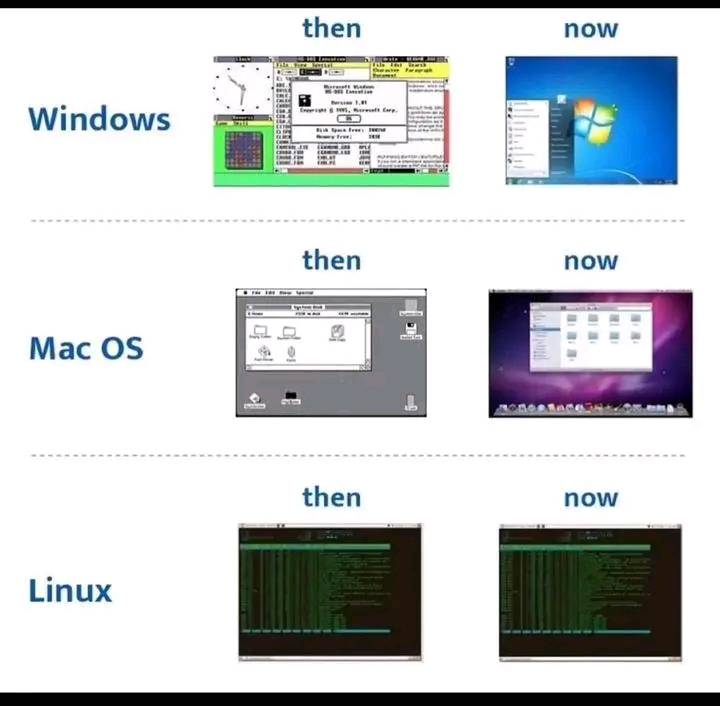
\includegraphics[scale=0.3]
    {./Presentations-pictures/Miscancellous-pictures/Evolution-of-operating-systems.jpg}

  \end{figure}

\end{frame}
% ######################################





% ######################################
\begin{frame}
  \frametitle{GNU/Linux i~po prostu Linux}


  Na~tych zajęciach będziemy~się starali używać nazw „GNU/Linux” i~„Linux”
  w~dość ścisłym sensie. Różnica ta bierze~się z~dość zawiłego problemu,
  mianowicie, co dany system operacyjny tak właściwie zawiera w~sobie?
  Wyjaśnimy to w~pewnym momencie bardziej dokładnie, na razie nie muszą~się
  Państwo w~ogóle przejmować tymi zawiłościami informatycznymi.

  Ponieważ życie nie może być proste, czasem będziemy mówili o~systemie
  Unix, na~podstawie którego Linux został zaprojektowany. Tym również nie
  muszą~się Państwo na razie przejmować.

\end{frame}
% ######################################





% ######################################
\begin{frame}
  \frametitle{Jak zdobyć system GNU/Linux?}


  Zdobycie umiejętności obsługi systemu GNU/Linux wymaga, jak łatwo~się
  domyślić, odpowiedniej liczby godzin spędzonych na pracy z~nim. Należy
  więc wspomnieć, że istniej przynajmniej kilka sposobów w~jaki mogą
  korzystać Państwo z~systemu GNU/Linux w~domu.

  Można go zainstalować na danym komputerze jako jedyny system operacyjny
  dostępny na nim. Można też zainstalowanie go jako drugiego systemu
  operacyjnego na danym komputerze, tak że uruchamiając komputer będziemy
  mieli do wyboru, czy chcemy korzystać z~systemu GNU/Linux, czy Windows
  (przykładowo). Można też korzystać zdalnie z~komputerów uczelnianych, za
  pomocą systemu Artemis. Możliwe jest też zainstalowanie GNU/Linuxa na
  komputerze z~systemem Windows, choćby korzystając z~\textsc{wsl} (Windows
  Subsystem for Linux). Ta lista nie wyczerpuje wszystkich możliwości
  korzystania z~tego systemu operacyjnego u~siebie w~domu.

\end{frame}
% ######################################





% ######################################
\begin{frame}
  \frametitle{Jak zdobyć system GNU/Linux?}


  Osoba, która chce dysponować u~siebie systemem GNU/Linux, powinna wybrać
  ten sposób używania go, który jej najbardziej odpowiada. Z~punktu widzenia
  podstaw pracy z~tym systemem, wybranie jednego bądź drugiego sposobu nie
  ma wielkiego znaczenia.

  Jeśli ktoś z~Państwa chce mieć u~siebie system operacyjny GNU/Linux i~ma
  problem z~wyborem sposobu korzystania z~niego, lub dokonał już wyboru,
  ale ma problem z~uruchomieniem go wybranym sposobem, to prosimy by
  zwrócić~się do nas w~tej sprawie. Można to zrobić bezpośrednio, lub
  pisząc pod adres \email.

  W~przypadku e-maila proszę mu nadać tytuł, który informuje o~treści
  wiadomości, jak \textit{Prośba o~pomoc w~zainstalowaniu systemu
    GNU/Linux}. Zwykle
  dostajemy dużo wiadomości z~zadaniami domowymi, jedna więcej o~niewiele
  mówiącym tytule \textit{Systemy operacyjne} łatwo nam umknie, a~wszak
  wymaga ona szybkiej odpowiedzi. To naprawdę dla nas ważne, dlatego
  powtórzymy to jeszcze parę razy.

\end{frame}
% ######################################





% ######################################
\begin{frame}
  \frametitle{Zadawanie pytań}


  Na zajęciach nie tylko można, ale \alert{należy} zadawać pytania
  na~dowolne związany z~nimi temat. W~szczególności \alert{należy} zadawać
  pytania, jeśli coś jest niezrozumiałe albo niejasne. Ten kurs ma być
  wstępem do systemu operacyjnego GNU/Linux, \alert{nie} zakładamy, że~są
  Państwo jego doświadczonymi użytkownikami. Byłoby to bardzo
  niewłaściwe założenie.

  Proszę pamiętać, że~gdy chodzi o~tematy związane z~zajęciami \alert{nie}
  ma pytań zbyt elementarnych czy głupich. Są~tylko niezadowalające
  odpowiedzi udzielane na~Państwa pytania. Jesteśmy tutaj by Państwu pomóc
  w~zaznajomieni~się z~pracą z~systemem operacyjnym na poziomie głębszym,
  niż ten napotykany przez większość użytkowników na co dzień.
  Pytania z~Państwa strony bardzo ułatwiają nam to zadanie. Zadawanie pytań
  nie oznacza, że~ktoś czegoś nie umie, tylko że~chce~się czegoś nauczyć.

\end{frame}
% ######################################





% ######################################
\begin{frame}
  \frametitle{Będziemy wiele upraszczać}


  Pytanie można i~\alert{należy} zadawać w~trakcie zajęć, po zajęciach, jak
  też pisząc na adres \email. Przy pisaniu na e-maila prosimy o~nadawanie
  tytułów postaci \textit{Pytanie o~X}, \textit{Pytanie z~przedmiotu
    „Systemy operacyjne”},~etc. Nie chcemy by tego typu wiadomości zginęły
  wśród wielu innych, które mogą poczekać trochę dłużej, a~brak dobrego
  tytuły niestety często do tego prowadzi. Proszę mieć pewną wyrozumiałość
  dla nas w~tym względzie.

  Pytania typu „Jaki oceniam obecny kierunek rozwoju gry \textit{Path~of
    Exile~2}?” musimy jednak zostawić na~czas po zajęciach.

  Ten kurs jest tylko \alert{wstępem} do~systemów operacyjnych. Ze~względu
  na rozmiar i~poziom skomplikowania tej dziedziny, dużą liczbę rzeczy
  będziemy musieli \alert{upraszczać}. Proszę więc pamiętać, że~choć
  staramy~się przekazywać rzetelną wiedzę, to to co mówimy będzie w~wielu
  wypadkach bardzo mocny \alert{uproszczeniem} rzeczywistości.

  % Sprawi nam dużą radość, jeśli ktoś będzie chciał zagłębić~się
  % w~tą tematykę i~w~takiej sytuacji służymy całą naszą wiedzą. Proszę~się
  % do nas zgłosić bezpośrednio, lub napisać e-maila, z~odpowiednim tytułem,
  % pod adres \email.

\end{frame}
% ######################################





% ######################################
\begin{frame}
  \frametitle{Jeśli ktoś chce się bardziej zagłębić w~temat}


  Sprawi nam dużą radość, jeśli ktoś będzie chciał zagłębić~się
  w~tematykę systemów operacyjnych i~w~takiej sytuacji służymy całą naszą
  wiedzą. Proszę~się do nas zgłosić bezpośrednio, lub napisać e-maila,
  z~odpowiednim tytułem, pod adres \email.

\end{frame}
% ######################################










% ################################################
\section{Podstawy GNU/Linuxa: włączanie powłoki}
% ################################################


% ######################################
\begin{frame}
  \frametitle{Powłoka BASH}

  \vspace{-0.5em}


  \begin{figure}

    \label{fig:BASH-shell}

    \centering


    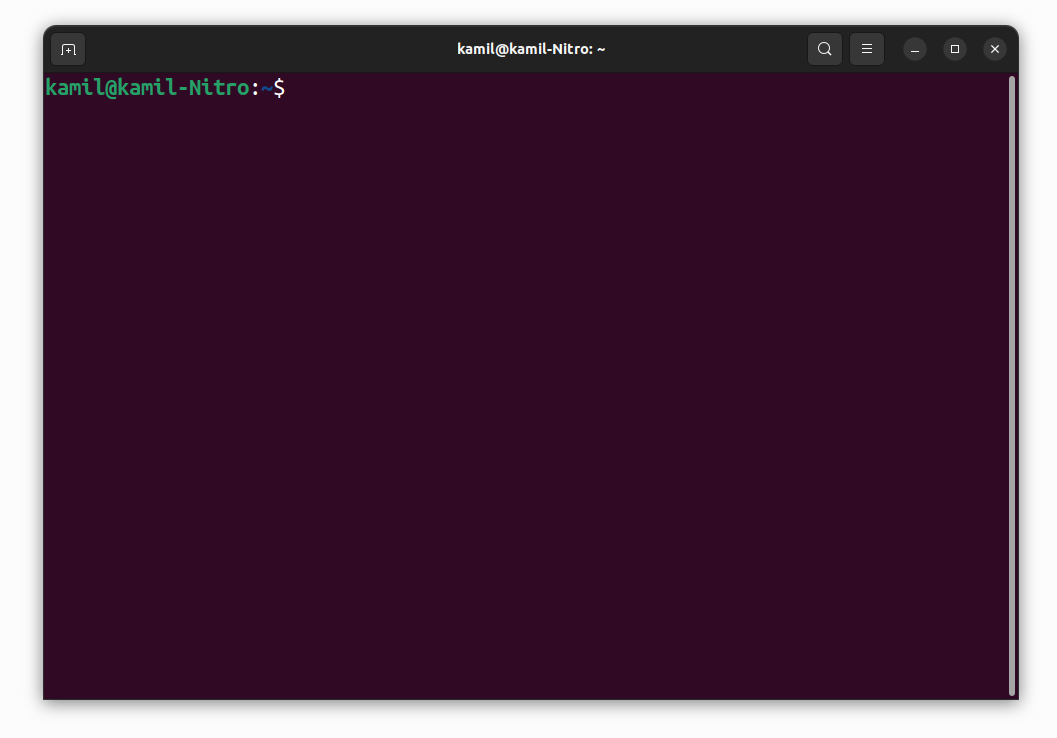
\includegraphics[scale=0.23]
    {./Presentations-pictures/Miscancellous-pictures/BASH-shell.png}


    \caption{Przykładowy wygląd włączonej powłoki \textsc{bash}, naszego
      głównego narzędzia pracy na tym przedmiocie.}

  \end{figure}

\end{frame}
% ######################################





% ##################
\begin{frame}
  \frametitle{Postęp technologiczny}

  \vspace{-0.5em}


  \begin{figure}

    \label{fig:Evolution-of-OS}

    \centering


    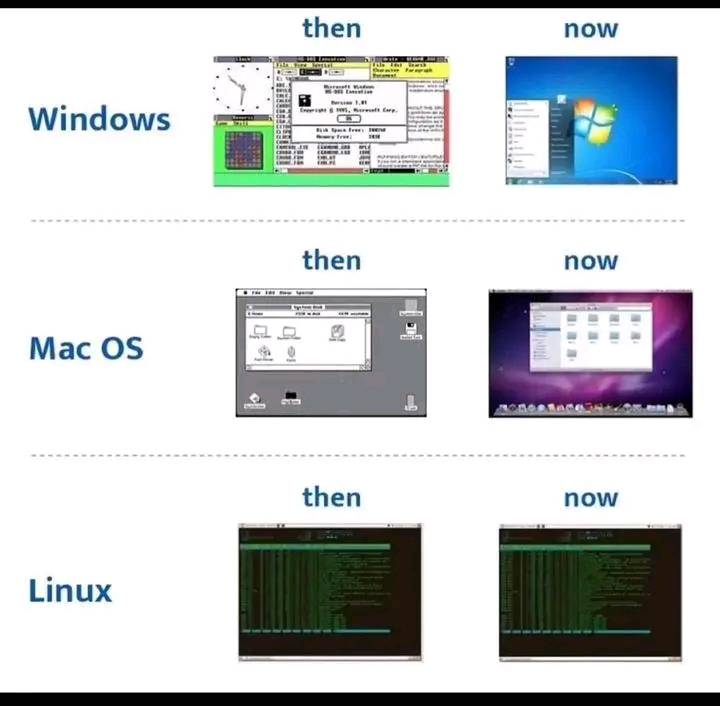
\includegraphics[scale=0.3]
    {./Presentations-pictures/Miscancellous-pictures/Evolution-of-operating-systems.jpg}

  \end{figure}

\end{frame}
% ##################





% ##################
\begin{frame}
  \frametitle{Włączanie powłoki}


  Naszym główny narzędziem na tych zajęciach będzie powłoka \textsc{bash}.
  Jej włączenie na samym początku potrafi być bardzo niewdzięcznym zadaniem,
  proszę spróbować to teraz zrobić. W~pierwszym kroku proszę wcisnąć
  \texttt{Ctrl-Alt-t} i~zobaczyć, czy powłoka~się otworzyć.

  Jeśli to nie zadziała, to proszę pochodzić kursorem po ekranie,
  aż~znajdziemy okienko „Szukaj”, „Wyszukaj”, etc. Proszę tam wpisać
  „Terminal”, „Konsola” lub „Consol” i~zobaczyć, czy wyświetli~się
  odpowiednia ikona. O~tym czy~się różni pojęcie „powłoki” od „terminala”
  czy „konsoli” może powiem później. Nie jest to jakaś szczególnie ważna
  rzecz na kursie wprowadzającym.

  Dlaczego używamy tak topornego i~niewdzięcznego narzędzia jak powłoka?
  Bo daje nam ona ogromne możliwości kontroli systemu operacyjnego, które
  są w~zasadzie niedostępne innymi drogami. Temat ten postaram~się rozwinąć
  w~przyszłości.

\end{frame}
% ##################










% ################################################
\section{Zajęcia, konsultacje}
% ################################################


% ######################################
\begin{frame}
  \frametitle{Charakter zajęć}


  Wykład zwykle ma bardziej charakter teoretyczny, a~te zajęcia bardziej
  \alert{praktyczny}. Pewna ilość teorii musi~się tu pojawić,
  ale~będziemy~się starali ją minimalizować. Chcemy jednak by te zajęcia
  były oparte na \alert{robieniu} czegoś, nie na słuchaniu. Wydaje~się nam,
  że~nawet jeśli to co robimy nie jest w~danej chwili zbyt ciekawe, to
  jednak lepiej coś samemu robić, niż kogoś słuchać.

  Możemy ustalić jeden termin na konsultacje, ale nasze doświadczenie mówi,
  że~to nie jest dobry pomysł. W~zasadzie nikt wtedy nie przychodzi, a~my
  wyznajemy zasadę, że~konsultacje są dla Państwa, a~nie dla nas. Jeśli
  Państwo chcą wyznaczenia takiego terminu, to najlepiej byłoby, gdy Państwo
  wspólnie wybrali konkretny czas, a potem przesłali nam informację
  o~swoim wyborze.

\end{frame}
% ######################################





% ######################################
\begin{frame}
  \frametitle{Konsultacje}


  Każda osoba, zawsze można umówić~się z~nami na~konsultacje indywidualne,
  choćby pisząc na~adres \email. Ponawiamy prośbę o~nadawanie e-mailom
  tytułów typu \textit{Prośba o~konsultacje}, \textit{Konsultacje
    z~przedmiotu „Systemy operacyjne”},~etc. Konsultacje te mogą~się
  odbywać na~żywo, online, telefonicznie,~etc. Konsultacje~są dla Państwa,
  nie dla nas.

  Nie lubimy, gdy zajęcia robią~się zbyt poważne, nie przeginajmy jednak
  w~drugą stronę.

\end{frame}
% ######################################





% ######################################
\begin{frame}
  \frametitle{Zbyt poważne zajęć to nic dobrego, ale\ldots}

  \vspace{-0.5em}


  \begin{figure}

    \label{fig:Jak-to-bywa-na-zajeciach}

    \centering


    
\includegraphics[scale=0.42]
    {./Presentations-pictures/Miscancellous-pictures/Jak-to-bywa-na-zajeciach.jpeg}

  \end{figure}

\end{frame}
% ######################################





% ######################################
\begin{frame}
  \frametitle{Nagrywanie zajęć}


  Będziemy~się starali nagrywać na \textsc{ms}~Teamsach każde nasze
  spotkanie. Proszę nam o~tym ciągle przypominać, bo jesteśmy dość
  roztrzepani i~któregoś razu na pewno o~tym zapomnimy.

  Proszę nam też zwracać uwagę, że~na ekranie czegoś nie widać,
  że~czcionka jest za mała, że~kolory kłują w~oczy, że~nagrany dźwięk
  jest niskiej jakości,~etc. Zajęcia są dla Państwa, naszym obowiązkiem jest
  dostarczyć Państwu najlepszej jakości materiały do nauki jakie jesteśmy
  w~stanie w~danej chwili stworzyć.

  % ZOSTAW!!!!
  % Niestety, jakość dźwięku to coś, na co mamy mały wpływ. Mogę~się starać
  % mówić możliwie blisko mikrofonu, ale nie wiem co więcej mogę zrobić.
  % Poza tym, na~pewno nie wyjdzie zbyt dobrze, bo te zajęcia często wymagają
  % bym~się poruszał, poza tym w~którymś momencie na pewno o~tym zapomnę.
  % Swoje uwagi na temat jakości nagrań proszę kierować do ludzi
  % odpowiedzialnych za~sprawy studenckie na \textsc{wsz}i\textsc{b}ie.

\end{frame}
% ######################################










% ######################################
\section{Zaliczenie przedmiotu}
% ######################################


% ##################
\begin{frame}
  \frametitle{Sposób uzyskania zaliczania}


  Z tego przedmiotu można uzyskać zaliczenie zaoczne, proszę~się w~tej
  sprawie zwrócić do~nas, osobiście lub piszą pod podany już kilkakrotnie
  adres \email. Jak poprzednio, prosimy o~nadanie e-mailowi nazwy,
  tłumaczącej jego treść.

  Normalnie, zaliczenie zdobywa~się na podstawie dwóch rzeczy:

  \vspace{-0.3em}



  \begin{itemize}

  \item prac domowych;

  \item dwóch sprawdzianów na żywo.

  \end{itemize}

  \vspace{-0.3em}



  Za prace domowe wystawiana jest jedna ocena, za~każdy ze sprawdzianów
  jedna oceny, przy czym ocena za~prace domowe, stanowi \alert{połowę}
  oceny końcowej. Dokładniej, ocena końcowa jest liczona jako średnia
  ważona: \\[0.3em]
  $\displaystyle
  \text{ocenaKońcowa} =
  \frac{ \text{ocenaSpraw1} + \text{ocenaSpraw2} +
    2 \cdot \text{ocenaPraceDom} }{ 4 }$,

  \vspace{0.5em}


  gdzie $\text{ocenaSpraw1}$ i~$\text{ocenaSpraw2}$ to dwie oceny ze
  sprawdzianów, zaś $\text{ocenaPraceDom}$ to ocena z~prac domowych.

  % za oddane prace domowe oraz
  % zaliczone sprawdziany. Sposób wyliczania oceny końcowej jest niestety dość
  % skomplikowany.
  % Wynika, to z~tego, że próbujemy znaleźć sposób oceniania, który promuje
  % regularną
  % pracę przez cały semestr, ale jednocześnie nie czyni sprawdzianów
  % rzeczami pozbawionymi znaczenia. Pragniemy też by sposób oceniani, nie był
  % też surowy wobec tych, którzy dobrze radzą sobie na początku semestru,
  % ale mają problem z~bardziej zaawansowanymi rzeczami. Wymyślenie czegoś
  % takiego nie jest łatwe.

  % ZOSTAW!!!!!
  % Zastanawiam~się czy nie dodać do tego projektu zaliczeniowego, ale są
  % pewne problemy techniczne, które stoją nam na drodze. Na dzień dzisiejszy
  % proszę przyjąć, że~projekt zaliczeniowego w~tym semestrze nie będzie.

\end{frame}
% ##################





% ######################################
\begin{frame}
  \frametitle{Sprawdziany na żywo}


  Ze względu na~zasoby dostępne w~internecie i~\textsc{ai}, koniecznością
  jest testowanie Państwa umiejętności na żywo. W~tym celu dwa razy
  przeprowadzimy sprawdziany na żywo. Terminy tych sprawdzianów prześlemy
  Państwu drogą elektroniczną.

  Żeby uzyskać zaliczenie z~przedmiotu, trzeba być \alert{osobiście}
  i~\alert{na żywo} na co najmniej jednym z~tych sprawdzianów i~uzyskać
  z~niego ocenę co najmniej~$3.0$. Nie jest wymagana obecność na żywo na
  \alert{obu} sprawdzianach, jeśli jednak ktoś pisze sprawdzian zdalnie
  i~nie przesłał usprawiedliwienia, to~może otrzymać najwyżej ocenę $3.0$.

  Jest to tak ważne, że~warto to powtórzyć kilkakrotnie. Aby uzyskać
  zaliczenie z~zajęć \textit{Systemy operacyjne}, trzeba być
  \alert{osobiście} na jednym z~dwóch sprawdzianów i~uzyskać z~tego
  sprawdzianu ocenę co najmniej~$3.0$. Nie jest ważne, czy ktoś będzie
  osobiście na pierwszym czy drugim sprawdzianie.

\end{frame}
% ######################################





% ######################################
\begin{frame}
  \frametitle{Sprawdziany na żywo}


  Jeszcze raz. Internet i~\textsc{ai} wymuszają na nas prowadzenie
  sprawdzianów na żywo i~każdy ma obowiązek być na żywo na \alert{jednym}
  z~nich. Jeśli ktoś już napisał jeden sprawdzian na żywo lub jest
  przekonany, że~będzie mógł napisać drugi z~nich na żywo, to może
  przynieść zwolnienie z~obecności
  na \alert{jednym} sprawdzianie. W~takiej sytuacji może napisać go zdalnie
  bez ponoszenia kary lub pisać na żywo w~innym terminie.

  Powody dla których można~się zwolnić z~obecności na żywo
  na~\alert{jednym} sprawdzianie są takie jak można podejrzewać:
  ważne sprawy rodzinne, konieczność bycia w~pracy, choroba,~etc.
  Jeśli ktoś pisze sprawdzian \alert{zdalnie} i~\alert{nie} dostarczył
  usprawiedliwienia, to nie ma możliwość uzyskania oceny wyższej niż~$3.0$.

  Dla osób które nie będą mógł być na żywo na żadnym z~proponowanych
  terminów, zorganizujemy jeden lub więcej dodatkowych.

\end{frame}
% ######################################





% ######################################
\begin{frame}
  \frametitle{Sprawdziany na żywo}


  Każdy sprawdzian składać~się będzie z~kilku zadań, których rozwiązanie
  należy zapisać w~pewnym pliku i~wysłać pod wspomniany adres \email.
  Za każde zadanie przyznawana jest pewna liczba punktów, ocena wystawiana
  jest na podstawie sumy zdobytych punktów, według poniższej skali.

  \begin{itemize}

  \item $40\%$ i~mniej~-- ocena dopuszczająca ($2.0$).

  \item $41\%\text{--}50\%$~-- ocena dostateczna ($3.0$).

  \item $51\%\text{--}60\%$~-- ocena plus dostateczna ($3.5$, $3+$).

  \item $61\%\text{--}80\%$~-- ocena dobra ($4.0$).

  \item $80\%\text{--}90\%$~-- ocena puls dobry ($4.5$, $4+$).

  \item $91\%\text{--}100\%$~-- ocena bardzo dobry ($5.0$).

  \end{itemize}

  Jeśli wynik wymaga zaokrąglenia, to zawsze zaokrąglamy na korzyść
  studenta. Czyli $40.1\%$ zaokrąglamy do $41\%$.

\end{frame}
% ######################################





% ######################################
\begin{frame}
  \frametitle{Prace domowe}


  Za pisanie sprawdzianu \alert{zdalnie} i~\alert{bez usprawiedliwienia},
  tracą Państwo od razu tyle punktów, że~nie jest możliwe otrzymanie oceny
  wyższej niż $3.0$.

  Sprawdziany można oczywiście poprawiać. Terminy sprawdzianów poprawkowych
  będziemy ustalać na bieżąco.

  Przejdźmy do prac domowych. Każdy zestaw takich prac składa~się
  z~kilku zadań, za każde z~nich można otrzymać odpowiednią liczbę punktów.
  Rozwiązanie danego zadania należy zapisać w~odpowiednim pliku i~przesłać
  na adres \email. Dokładniej te kwestie będą omówione w~pliku zawierającym
  zadania.

  Prace domowe proszę \alert{spróbować} potraktować nie jako ciężki
  obowiązek do odhaczenia, tylko jako możliwość nauczenia~się czegoś
  w~praktyce. Tak, wiemy, łatwo~się mówi, żeby nie traktować tego jako
  ciężkiego obowiązku, a~w~rzeczywistości jest to trudne.

\end{frame}
% ######################################





% ######################################
\begin{frame}
  \frametitle{Prace domowe}


  Proszę jednak wiedzieć, że~prace domowe są zadawane w~pierwszym rzędzie
  po~to, żeby Państwo mogli~się czegoś nauczyli przy ich robieniu. Dopiero
  w~drugim rzędzie, by móc wystawić Państwu oceny. Jeśli Państwo oszukują
  przy oddawaniu tych zdań, to z~naszej perspektywy, oszukują Państwo przede
  wszystkim samych siebie.

  Prace domowe należy próbować rozwiązać możliwie samodzielnie. W~razie
  napotkania problemów nie tylko można,
  ale i~\alert{należy} prosić o~pomoc kolegów, korzystać z~materiałów
  w~internecie i~używać programów takich jak Chat\textsc{gpt}. Można też
  pisać do nas po adres~\email o~pomoc. Ale z~jakiegoś powodu, mało kto
  prosi o~taką pomoc. Dziwne ;).

  W~semestrze należy~się spodziewać $5$~zestawów prac domowych, acz ich
  dokładna liczba będzie zleżeć od~tego, jak wszystko będzie przebiegać
  w~praktyce.

\end{frame}
% ######################################





% ######################################
\begin{frame}
  \frametitle{Prace domowe}


  Pod koniec semestru punkt zdobyte za prace domowe zostaną zsumowane
  i~wystawiona zostanie za nie \alert{pojedyncza} ocena według tej samej
  skali co poprzednio.

  \begin{itemize}

  \item $40\%$ i~mniej~-- ocena dopuszczająca ($2.0$).

  \item $41\%\text{--}50\%$~-- ocena dostateczna ($3.0$).

  \item $51\%\text{--}60\%$~-- ocena plus dostateczna ($3.5$, $3+$).

  \item $61\%\text{--}80\%$~-- ocena dobra ($4.0$).

  \item $81\%\text{--}90\%$~-- ocena puls dobry ($4.5$, $4+$).

  \item $91\%\text{--}100\%$~-- ocena bardzo dobry ($5.0$).

  \end{itemize}

  Jak poprzednio, wyniki zaokrąglenia na korzyść studenta. Czyli $40.1\%$
  zaokrąglamy do $41\%$.

\end{frame}
% ######################################





% ######################################
\begin{frame}
  \frametitle{Ocena końcowa}


  Staram~się tak układać punktację, żeby trudniejsze zadania z~prac
  domowych były wyżej punktowane, a~ponieważ trudniejsze zadania są zwykle
  w~późniejszych zestawach zadań, więc proszę wziąć pod uwagę, że~te
  późniejsze zestawy będą prawdopodobnie wyżej punktowane. Osiągnięcie
  tego jest jednak trudne, więc czas pokaże jak to naprawdę wyjdzie.

  Jak już mówiliśmy, ocenę końcową wystawiamy na podstawie ocen
  ze~sprawdzianów i~oceny z~prac domowych. W~przypadku oceny końcowej,
  zawsze jest możliwość jej poprawienia. W~tym celu proszę~się z~nami
  skontaktować, choćby pod adresem \email.

\end{frame}
% ######################################










% ################################################
\section{Materiały z~których korzystaliśmy}
% ################################################


% ######################################
\begin{frame}
  \frametitle{Materiały z~których korzystaliśmy}


  Przygotowując te zajęcia korzystaliśmy z~następujących materiałów.
  \alert{Lista wciąż nie jest kompletna.}

  Andrew S. Tanenbaum \textit{Systemy operacyjne. Wydanie~III},
  \parencite{Tanenbaum-Systemy-operacyjne-Wydanie-III-Pub-2013}.

  Vintage Computer Federation \textit{VCF East: Ken Thompson interviewed
    by~Brian Kernighan} \parencite{VCF-VCF-East-Ken-Thompson-interviewed-by-Brian-ETC-Ver-2019}.


\end{frame}
% ######################################





% ######################################
\begin{frame}
  \frametitle{Błędy w~materiałach}


  Prosimy by informować nas o~wszystkich błędach znalezionych w~naszych
  materiałach, najlepiej pisząc pod adres \email.

\end{frame}
% ######################################














% ################################################
\appendix
% ################################################





% ######################################
\EndingSlide{Dziękujmy! Pytania?}
% ######################################





% ####################################################################
% ####################################################################
% Bibliography

\printbibliography










% ####################################################################
% End of the document

\end{document}
